%
% File acl2018.tex
%
%% Based on the style files for ACL-2017, with some changes, which were, in turn,
%% Based on the style files for ACL-2015, with some improvements
%%  taken from the NAACL-2016 style
%% Based on the style files for ACL-2014, which were, in turn,
%% based on ACL-2013, ACL-2012, ACL-2011, ACL-2010, ACL-IJCNLP-2009,
%% EACL-2009, IJCNLP-2008...
%% Based on the style files for EACL 2006 by 
%%e.agirre@ehu.es or Sergi.Balari@uab.es
%% and that of ACL 08 by Joakim Nivre and Noah Smith

\documentclass[11pt,a4paper]{article}
\usepackage[hyperref]{acl2018}
\usepackage{times}
\usepackage{latexsym}
\usepackage{amsmath}
\usepackage{url}

\usepackage{tabularx}

\usepackage{titlesec}
\setcounter{secnumdepth}{3}

\usepackage{graphicx}
\graphicspath{ {graphics/} }

\aclfinalcopy % Uncomment this line for the final submission
%\def\aclpaperid{***} %  Enter the acl Paper ID here

%\setlength\titlebox{5cm}
% You can expand the titlebox if you need extra space
% to show all the authors. Please do not make the titlebox
% smaller than 5cm (the original size); we will check this
% in the camera-ready version and ask you to change it back.

\newcommand\BibTeX{B{\sc ib}\TeX}

\title{Movise Domain Bot \\ Final project}

\author{Andrea Tupini \\
  MAT.  194578 \\
  {\tt andrea.tupini@studenti.unitn.it}}

\date{}

\begin{document}
	
\maketitle

\begin{abstract}
	
	abstract. 
	\\
	
\end{abstract} 

\section{Introduction}

	This project consisted of building a bot that could answer questions on the movie domain. We had to build both the NLU and dialogue modules. In this report we'll see a bit how the bot works and the decision made during it's design, plus some encountered problems.
	
\section{Data Analysis}
\label{sec-data-analysis}
	
	The original data that was provided consisted of a movie database that contains various information on the movie domain and the data needed for training the NLU module of the bot (this was given in NLSPARQL format).
	
	\subsection{NLU Data}
	\label{ssec-nlu-data}
	
		Originally, the provided NLU data consisted of the following files: 
		
		\begin{description}
			\item[NLSPARQL.test] words and IOB tags for testing
			\item[NLSPARQL.train] words and IOB tags for training
			\item[NLSPARQL.test.utt.labels] contains labels on what each question in the test set is about              
			\item[NLSPARQL.train.utt.labels] labels on questions of training set
		\end{description}
	
		The NLSPARQL format is not recognized by Rasa, so these had to be converted to a properly formatted \textit{json} file. In the rasa format, for each sentence we need to provide which are the entities and intent of the sentence (entities and intents are defined in section \ref{ssec-nlu-module}). Extracting entities was just a simple matter of using the IOB tags that are not \textit{O}s, and the intents were taken directly from the \textit{labels} files.
		
		Here we have a graphic that shows the count of different entity types provided in the dataset (note that it is log scaled so as to account for the difference between the most common entity and the least common one):
		
		\hspace*{-0.4cm}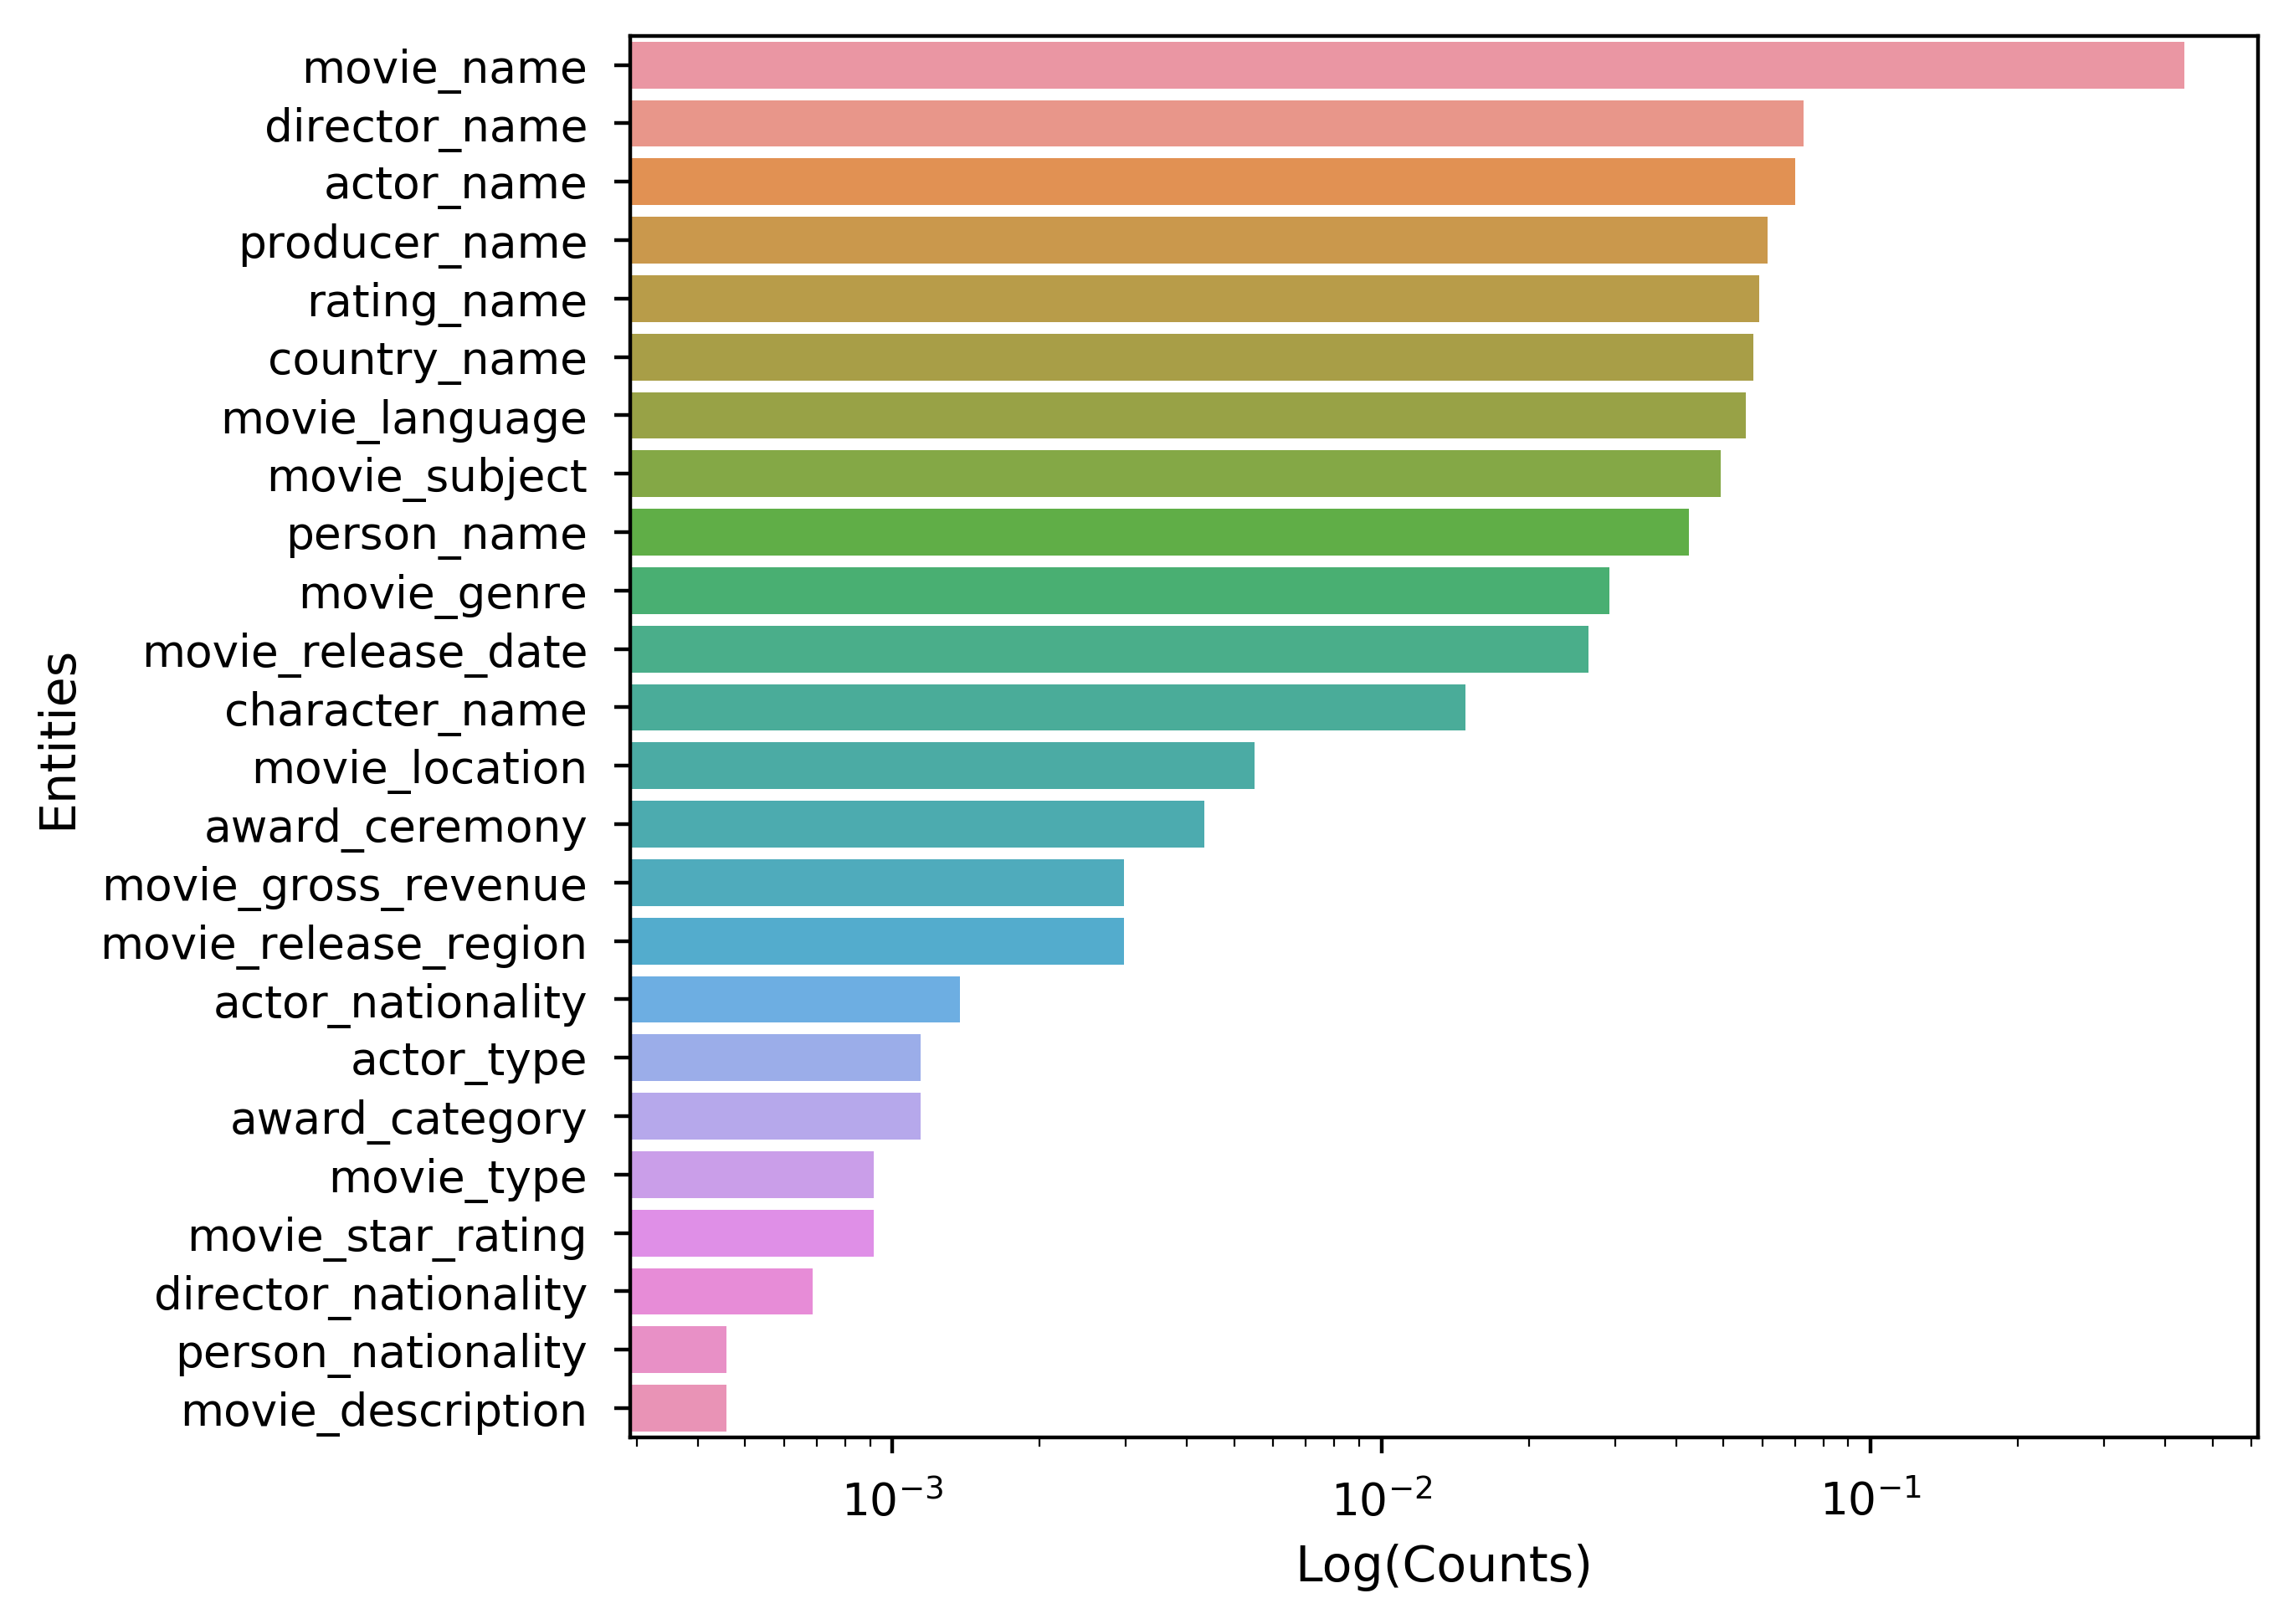
\includegraphics[scale=0.5]{entities_frequency}
		
		Here we can see that the \textit{movie name} entity is much more common than any of the other entities. But we do have a good amount of the entities we would expect our users to use the most, which is good so that the model is actually able to learn them.  
		
		Below is another graphic showing the count of intents (this has also been log scaled):
		
		\hspace*{-1.7cm}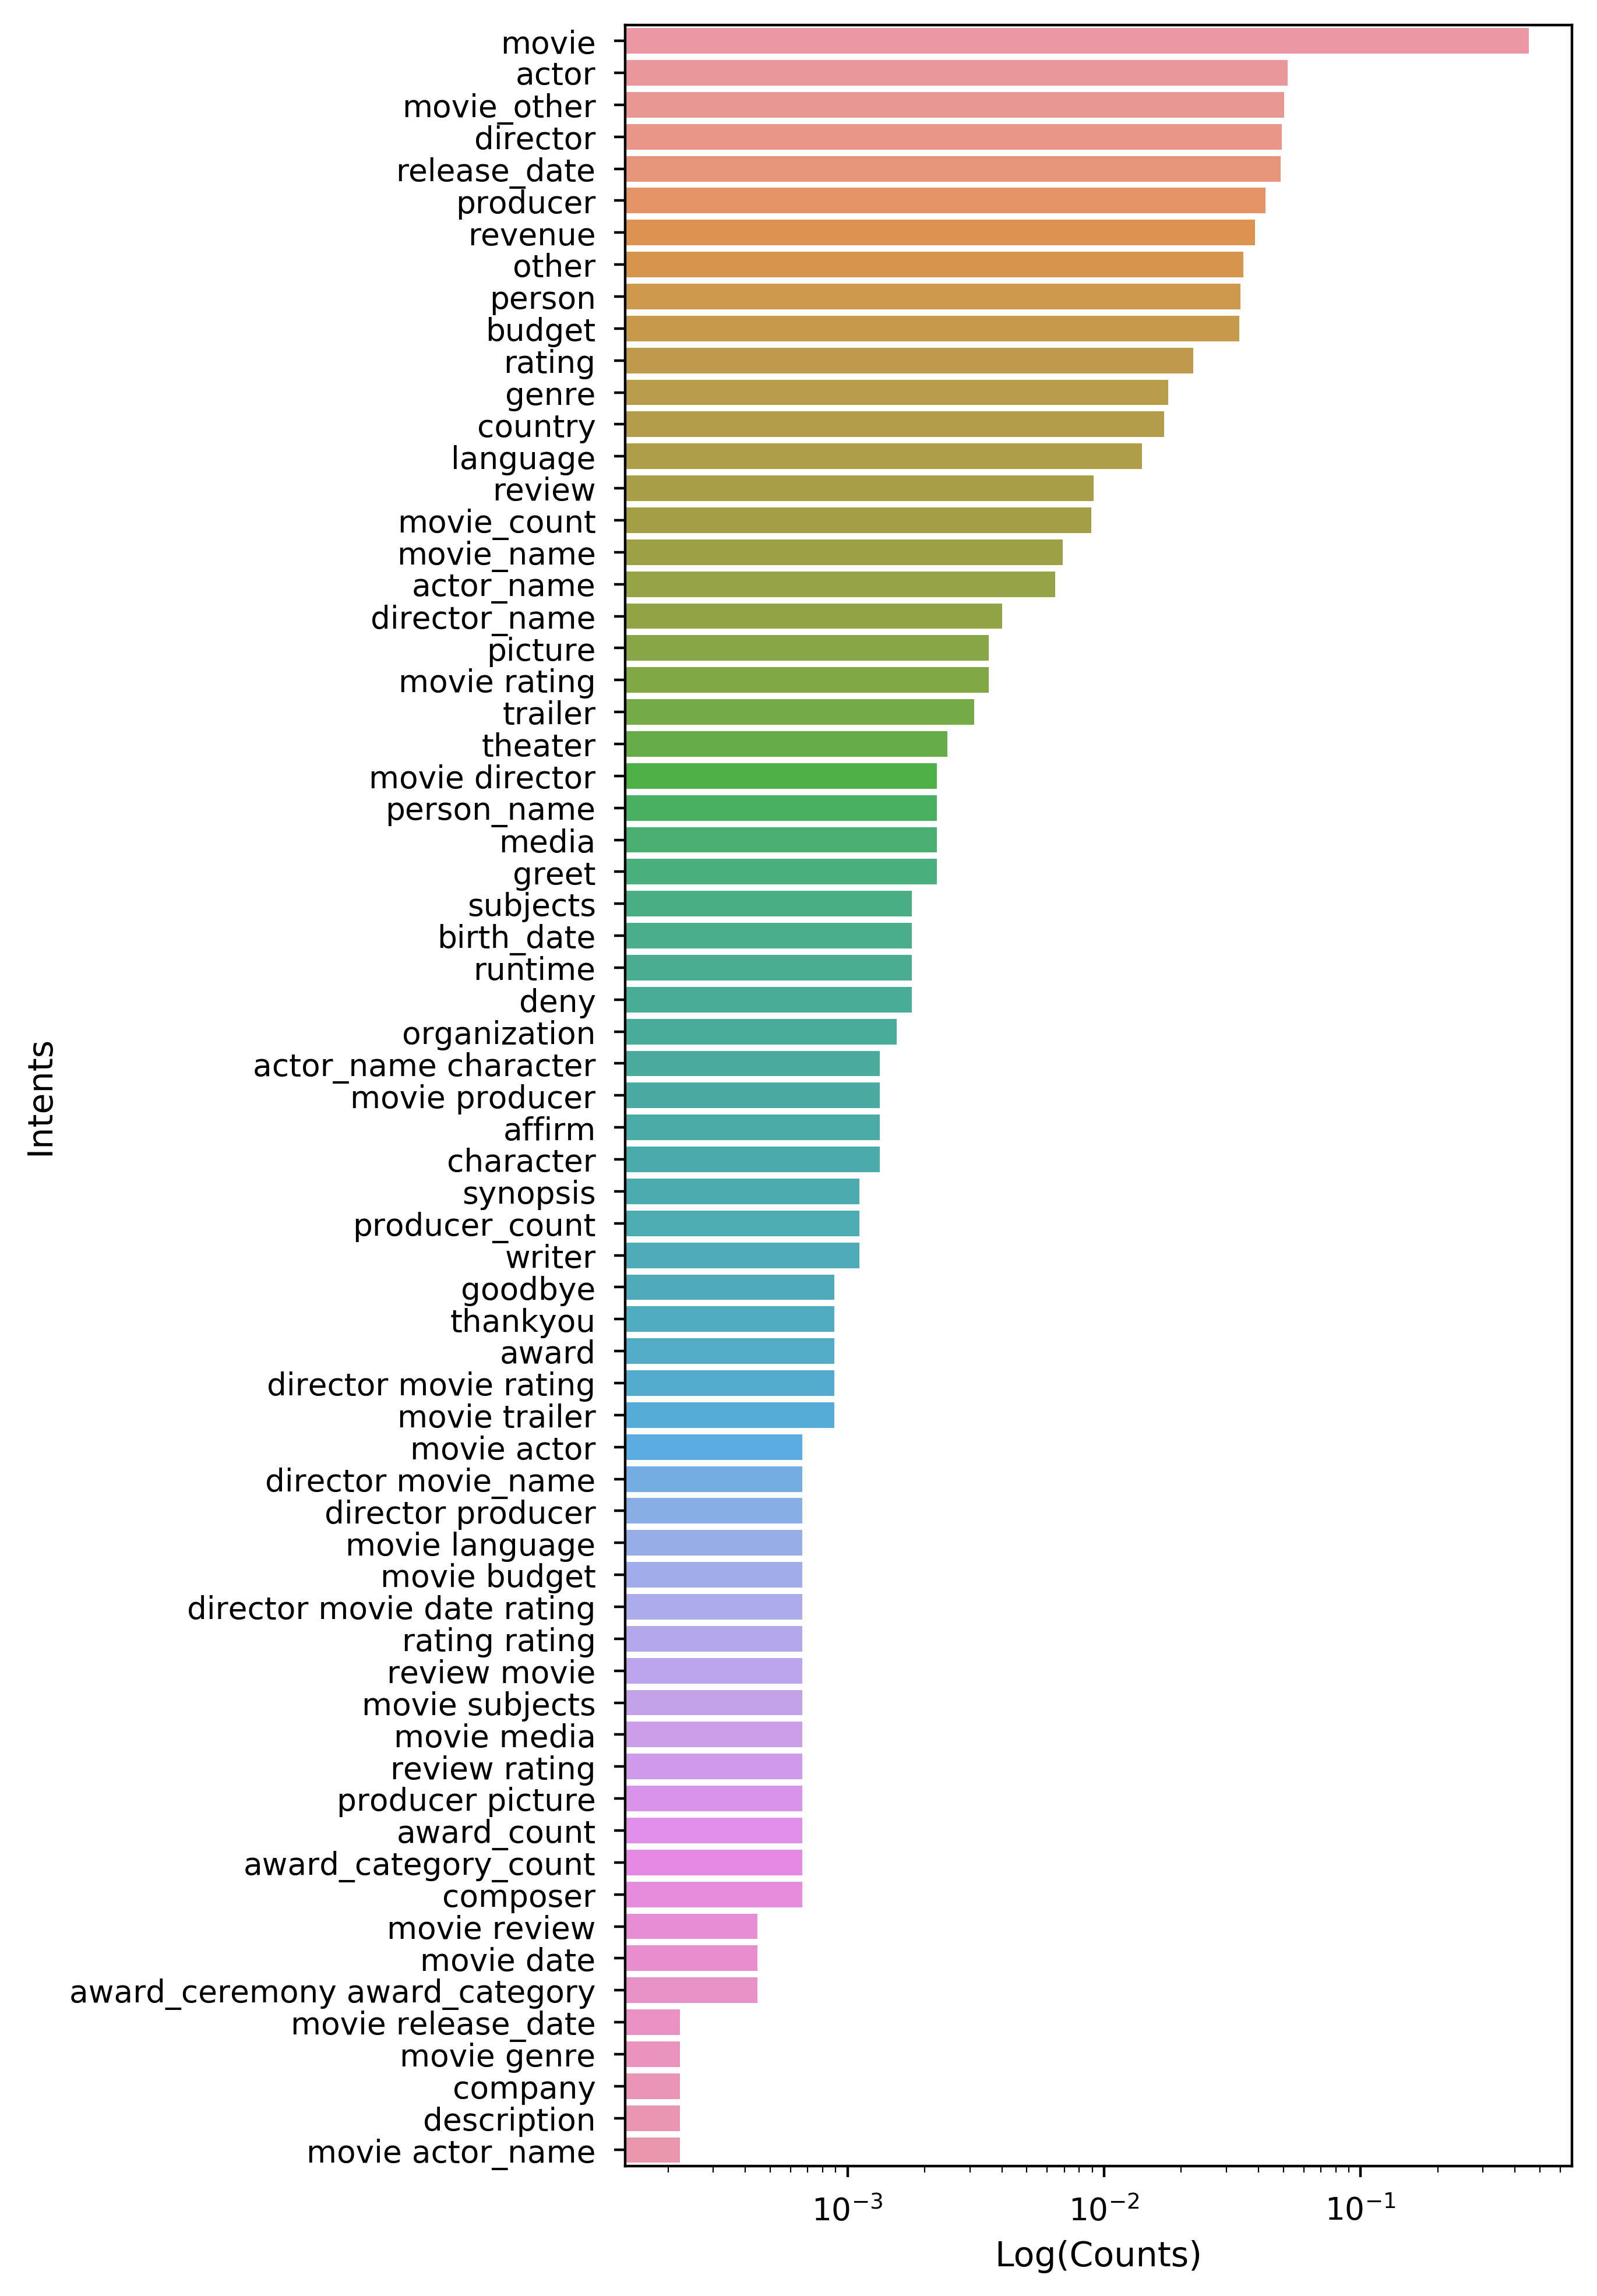
\includegraphics[scale=0.5]{intents_frequency}
		
		It is easy to note that also in this case \textit{movie} is the most common thing talked about. We can see that the difference between the most common item (\textit{movie}) and the least common one (\textit{movie actor name}) is much more pronounced for intents than it is for entities.
		
		Note that entity types may take many different values (for example, \textit{movie\_name} can be an entity representing diverse movie names in different sentences), while intents are always set (a sentence can only have one intent). This is the reason why we have much less entities than intents.
		
	
	\subsection{Database}
	\label{ssec-database}
		
		The database basically contains all the knowledge that the bot has on the movie domain. If something is asked of the bot that is now in the database then it won't be able to answer. Each row in the database contains the information for one movie and it has the following columns:
		
		\begin{itemize}
		\setlength\itemsep{-0.48em}
			\item Title 
			\item Actors
			\item Director
			\item Genres
			\item Country where it was made
			\item Release Date
			\item Original language
			\item Duration in minutes
			\item If it was released in color or not
			\item Budget
			\item Plot Keywords
			\item Gross Revenue
			\item IMDB core
			\item Likes on the Facebook movie page
			\item Link to the movie's IMDB page
		\end{itemize}

		
		The original database was fine, there were some empty columns but in those cases the bot will tell the user that it doesn't have the information to answer. However there was one issue that required to modify the database to fix it and it was that some rows had as \textit{release date} years that were not possible (ie: \textit{18000000}), so all of the publishing years above 2018 were deleted.


\section{Bot Modules}
\label{sec-bot-modules}

\subsection{NLU Module}
\label{ssec-nlu-module}

taslk about entities

\subsubsection{Rasa NLU}
\label{ssec-rasa-nlu}
	
	remember to talk about pipeline

\subsection{Dialogue Module}
\label{ssec-dialogue-module}

\subsubsection{Rasa Core}
\label{ssec-rasa-core}	

	remember to talk about domain

\subsubsection{Policies}
\label{ssec-policies}	

\subsubsection{Custom Actions}
\label{ssec-custom-actions}	

\subsubsection{Forgetting}
\label{ssec-forgetting}	

Not stremlined/goal otiented task.

\section{Evaluation}
\label{sec-evaluation}

	ev

\section{Speech}
\label{sec-speech}

	

\section{Difficulties}
\label{sec-difficulties}

	fw.

\section{Possible Improvements}

	One thing we can see in the entity counts graphic in \ref{ssec-nlu-data} is that we could actually join some of these entities toghether and so remove some entropy from the daataset.

\section{Conclusion}
\label{sec-conclusion}
	
	remember to add references to tools' sites
	


% include your own bib file like this:
\bibliographystyle{plain}
%\bibliography{acl2018}

%\bibliographystyle{plainnat}
\bibliography{bibliography}

%\bibliographystyle{acl_natbib}


\end{document}
